
\documentclass[
%reprint, %double column
%superscriptaddress,
%groupedaddress,
%unsortedaddress,
%runinaddress,
%frontmatterverbose, 
%preprint,
%preprintnumbers,
nofootinbib,
%nobibnotes,
%bibnotes,
 amsmath,amssymb,
 aps,
%pra,
%prb,
%rmp,
%prstab,
%prstper,
%floatfix,
]{revtex4-2}

\usepackage{scrextend}
\usepackage[bottom]{footmisc}
\usepackage{comment}
\usepackage{graphicx}% Include figure files
\usepackage{dcolumn}% Align table columns on decimal point
\usepackage{bm}% bold math
%\usepackage{hyperref}% add hypertext capabilities
%\usepackage[mathlines]{lineno}% Enable numbering of text and display math
%\linenumbers\relax % Commence numbering lines

%\usepackage[showframe,%Uncomment any one of the following lines to test 
%%scale=0.7, marginratio={1:1, 2:3}, ignoreall,% default settings
%%text={7in,10in},centering,
%%margin=1.5in,
%%total={6.5in,8.75in}, top=1.2in, left=0.9in, includefoot,
%%height=10in,a5paper,hmargin={3cm,0.8in},
%]{geometry}

\def\code#1{\texttt{#1}}

\begin{document}


\title{Distribution sampling with Normalizing Flows}
\thanks{Bayesian Statistical Methods and Data Analysis, FS2024}

\author{Nico H\"arringer}

 \email{haenico@ethz.ch}
\affiliation{ETH Z\"urich, Institute for Particle Physics and Astrophysics (IPA), Z\"urich, Switzerland}

\date{\today}

\begin{abstract}
In this report, I discuss the background of Normalizing Flow algorithms. A quick demonstration is made how sampling is possible when the considered distribution is a two-dimensional Gaussian. This report is made as part of the \textit{Bayesian Statistical Methods and Data Analysis} course (402-0738-10L) held by T. Tr\"oster in spring 2024.
\end{abstract}


\maketitle

\section{Introduction}
\subsection{Distribution sampling}

Often in Physics we have the problem that we have only a limited set of measurements. That could be for example due to the rarity of a given process or just because the detection method prevents you from getting a lot of samples. This poses an issue, since usually detectors or particle detection strategies are devised based on simulated events. For this reason it would be preferable to have access to the distribution a given process follows, such that we can generate as many events as we desire to complete our job. \\

In High Energy Physics for example, accurate modelling and sampling from very complex probability distributions are important for a variety of applications. Often, traditional ways of sampling from such a complex distribution quickly face the so-called curse of dimensionality which makes sampling practically impossible. \\

\subsection{Normalizing Flows}

Normalizing Flow (NF) algorithms as proposed by Rezende et al. \cite{NF} constitute a class of generative models used for the effective learning and sampling for typically intricate and multivariate distributions. Contrary to traditional Monte Carlo methods relying on direct sampling techniques, NF harness the power of neural networks to approximate the underlying distribution. Normalizing Flows involve parametrizing a transformation within the flow, enabling mapping of events from the data space (which can be complex) to a more simpler latent space. Such a mapping requires the usage of invertible transformations $f: \mathbb{R}^d \rightarrow \mathbb{R}^d$. Instead of a single transformation, it is common to compose the transfromation $f$ with multiple invertible transformations and chain them: $f := f_N \circ ... \circ f_1$. We are free to choose the number of transformations and it will go into the NF as a hyperparameter. \\ 

\begin{figure}[h!]
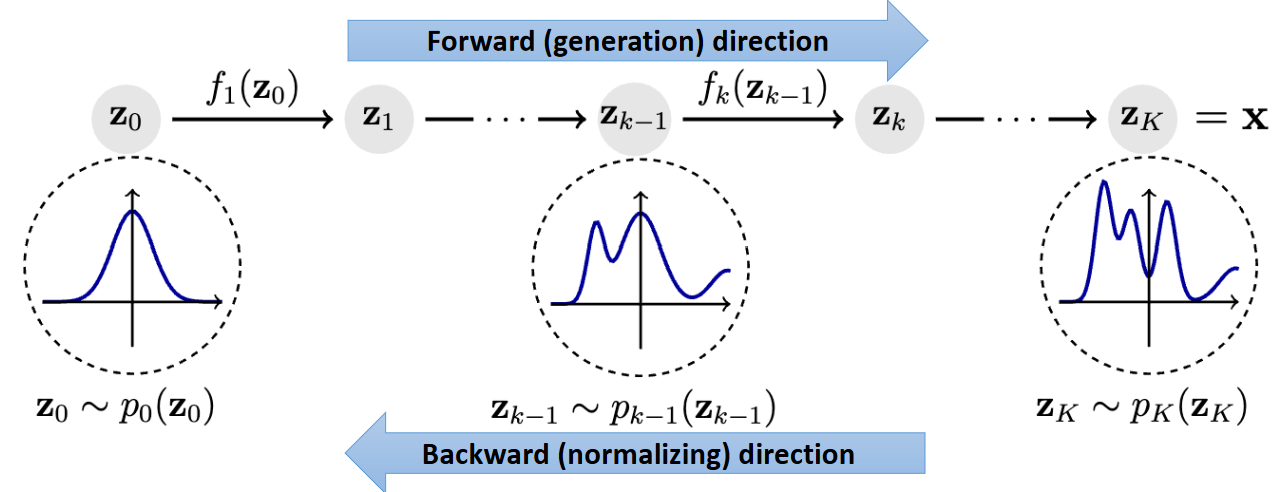
\includegraphics[scale=0.90]{Plots/NF_intro.png}
\caption{\label{fig:NF_intro} The concept of Normalizing Flows. We start with a complex distribution and apply a series of bijective transformations on it until we have a relatively easy distribution (i.e. Gaussian). Then, we can revert this chain of transformations and sample from a Gaussian our complex distribution. This Figure was taken from \cite{NF_Intro}. }
\end{figure}

\newpage

\section{Theory}
In the following chapter, the theory of NF is explained and an introduction into the two main flows of this report Neural Spline Flow (NSF) and Gaussianization Flows (GF) \cite{NSF, GF} is made.

\subsection{Normalizing Flows}
A center piece of Normalizing Flows is the usage of invertible functions, as already mentioned in the previous chapter. This allows us, given the function is chosen accordingly, a mapping from a complex data distribution to a simple, latent distribution. This latent distribution is a-priori not Gaussian. \\

\subsubsection{Algorithm}

An example NF flow algorithm is depicted in Fig. \ref{fig:NF_Explained}. First, we start with an input vector $\boldsymbol{x}$ which is split with a first function in two parts with the same dimension $\boldsymbol{x_1}$ and $\boldsymbol{x_2}$. The first part $\boldsymbol{x_1}$ is copied and goes through a freely chosen neural network. The choice of this neural net will influence the final result. The output of the neural net is a scale parameter $s$ and a translate parameter $t$. We do an affine transformation and apply the scaling and translation parameter to our second part of our input vector. The output of that is a modified $\boldsymbol{x_2}$ which is scaled on one hand and translated on the other: $\boldsymbol{z_2} := s \cdot \boldsymbol{x_2} + t$. The resulting vector $\boldsymbol{z_2}$ is then concatenated with the unmodified first part of the input vector: $\boldsymbol{z} = (\boldsymbol{x_1}, \boldsymbol{z_2})$. As a final step in this chain, the components of the vector $\boldsymbol{z}$ are shuffled and reused as an input vector of the chain. After enough iterations of this process, every part of the original vector had seen the neural net at least once. \\

\begin{figure}[h!]
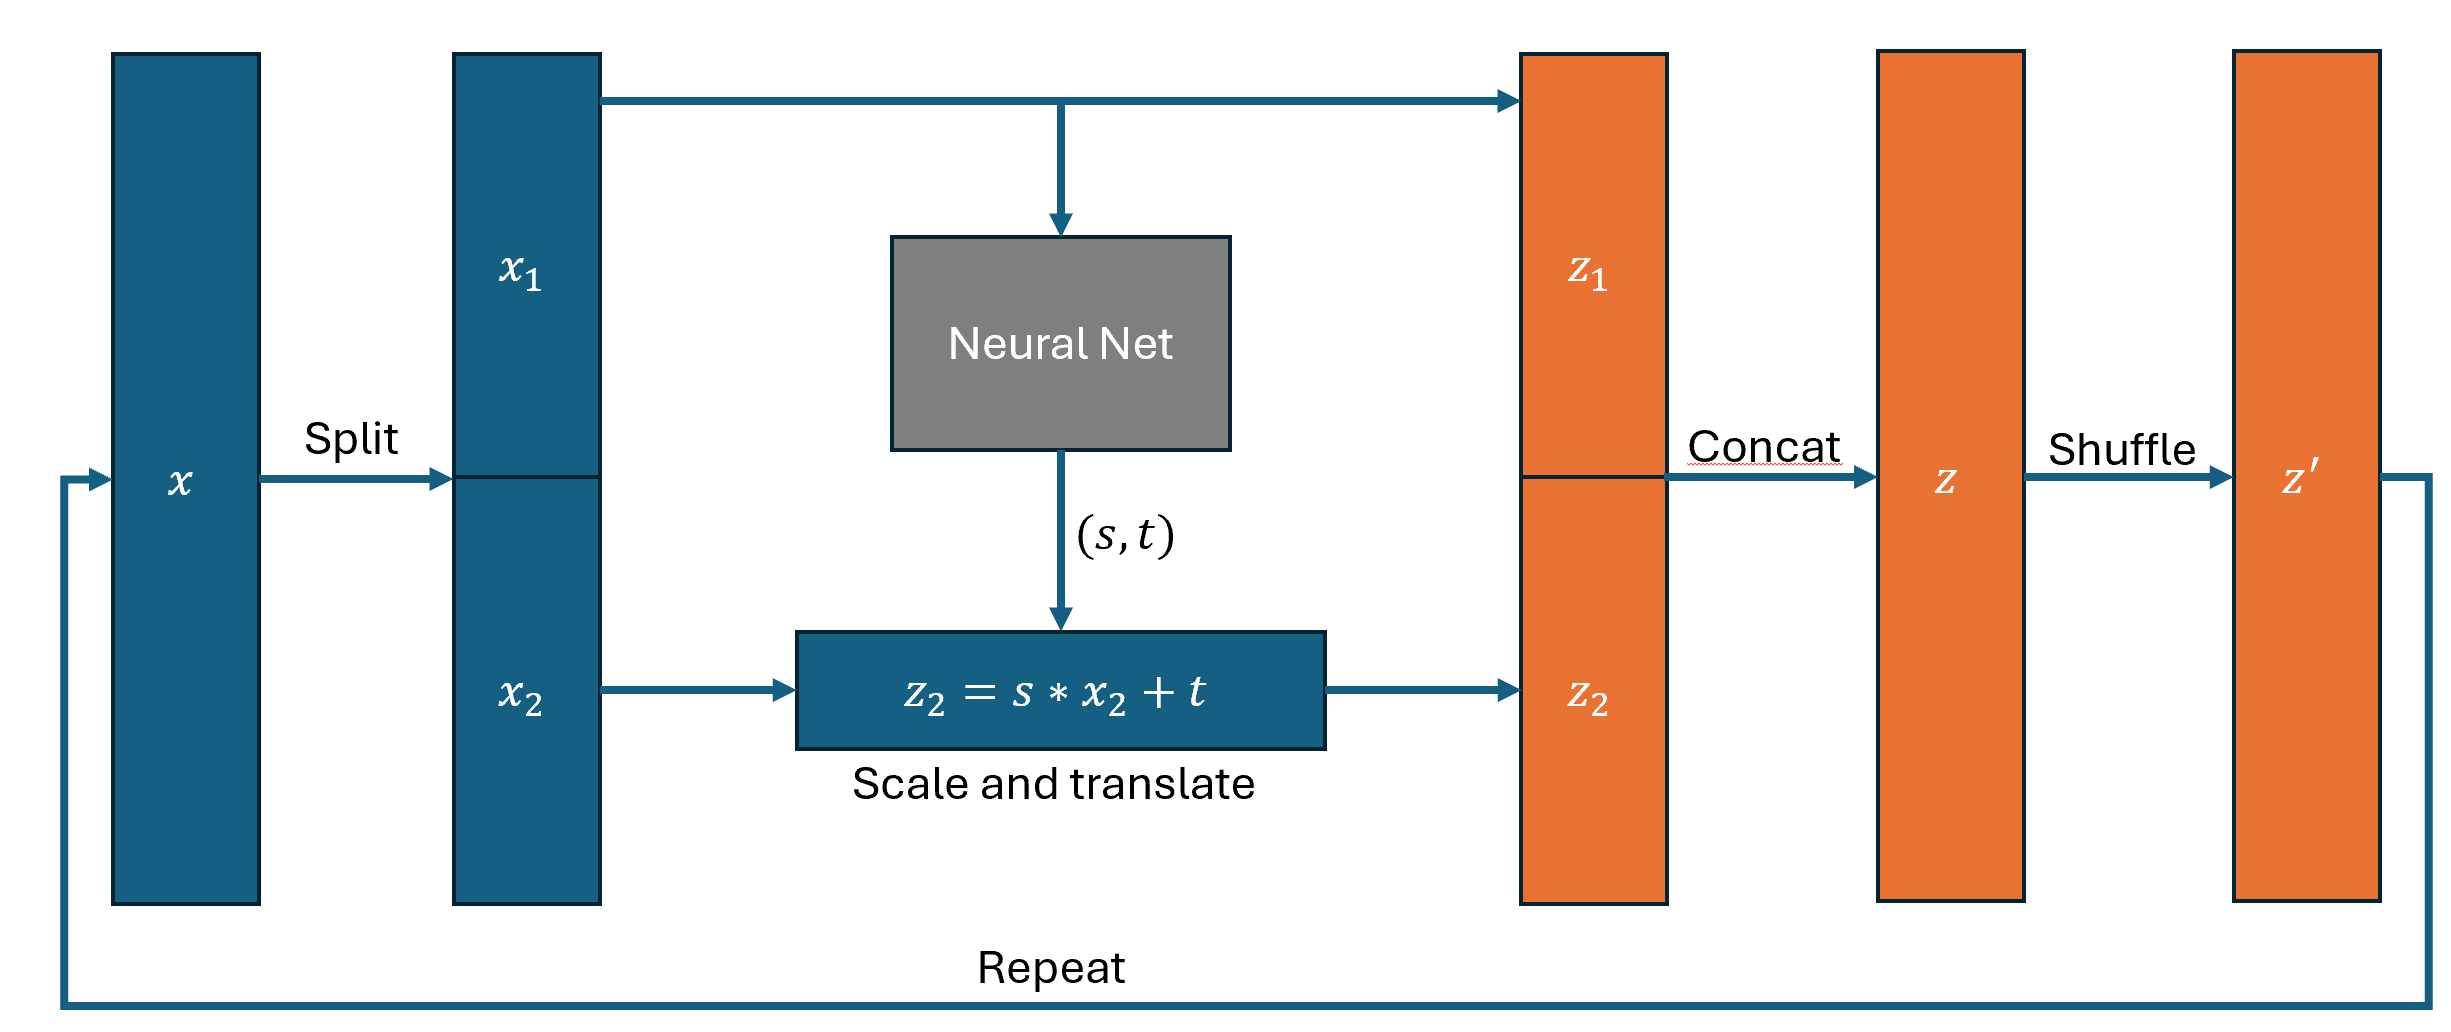
\includegraphics[scale=0.60]{Plots/NF_Explained.png}
\caption{\label{fig:NF_Explained} Explanation of the Normalizing Flow algorithm. The design of this Figure was taken from \cite{NF_YT}.}
\end{figure}

Through the invertibility of the functions used, we can go after the training process from the latent distribution back to the original one after applying the inverse. We reverse the chain, but not the neural net which is an advantage, since the inverse might not exist. 

\subsubsection{Loss function}
The loss function (also cost function) measures, how well a model's prediction match the actual data. They provide a quantitative way to adjust the model's parameters to minimize errors and improve the performance.

For Normalizing Flows we use maximum likelihood estimation. Essentially, we want to find the
\begin{equation}
    \mathrm{argmax}\ \mathrm{log}(p_{\boldsymbol{\theta}}(X)) = \sum_{i=0}^{m-1} \mathrm{log}(p_{\boldsymbol{\theta}}(x_i))
\label{eqn:loss}
\end{equation}.

Since we use invertible functions (in particular bijective ones), we can compute the exact likelihood and we find that $\mathrm{log}(p_{\boldsymbol{\theta}}(x_i)) = \mathrm{log}(p_{z}(f_{\boldsymbol{\theta}}(x_i))) + \mathrm{log}\ |\mathrm{det}D f_{\boldsymbol{\theta}}(x_i)|$. The extra term $\mathrm{log}\ |\mathrm{det}D f_{\boldsymbol{\theta}}(x_i)|$ comes from the fact, that we have a constraint from statistics, called the probability mass conservation. We have to require $\int p_x(x) dx = \int p_{z}(f(x)) dx$. By taking the derivative with respect to $x$, this leads to $p_x(x) = p_{z}(f(x)) \cdot |\mathrm{det}D f(x)|$. The full function is then maximized during training of the neural net.

\subsection{Neural Spline Flow (NSF)}

When we use a Neural Spline Flow (NSF) powered NF algorithm, we use splines to parametrize the invertible transformations. Splines are a powerful tool and we can use them to approximate almost every distributions. Mathematically they are smooth, piecewise polynomial functions. For the project, we used so-called monotonic rational-quadratic spline transformations. These splines can model complex distributions with a high degree of smoothness and flexibility. \\

The advantage of NSFs lie in their flexibility and are a good general flow. Since the transformations are smooth, they should converge relatively quickly and give stable gradients.

The disadvantage is, that they are computationally heavy compared to other flows (in particular the Gaussianization Flow). The computation of the splines take longer, since they are piecewise defined. Due to the high flexibility of the NSF, overfitting might become a problem for some models.

\subsection{Gaussianization Flow (GF)}
Gaussianization Flows are NF which transform the a-priori complex data distribution into a Gaussian distribution. Gaussianization is the process which aims to iteratively transform the data into a form that becomes progressively closer to a multivariate Gaussian.

The advantage of GF is their flexibility and efficiency, similar to the NSF. Their disadvantage is, that their performance is a function of the starting parameters. Properly tuning them is essential for the GF to be effective.

\section{Application}
In order to test the implementation of NF in Python and compare the different flow algorithms, we used a combination of \code{pytorch} \cite{PyTorch} and \code{zuko} \cite{zuko}. The latter is a Python package that implements NF in \code{pytorch}.

\subsection{Unimodal two-dimensional Gaussian}
To start off and to become familiar with the framework, we had a look at a standard, unimodal two-dimensional Gaussian function with the following parameters:

\begin{equation}
    \mu = \begin{pmatrix} 2 \\ -1 \end{pmatrix},\ \mathrm{\Sigma} = \begin{pmatrix} 1.0 & 0.7 \\ 0.7 & 1.0 \end{pmatrix}
\label{eqn:unimod}
\end{equation}

We created a dataset containing 1000 data points for training for each test using the same seed to allow for comparison. Since the distribution is two-dimensional, we created for each datapoint a x and y component, as well as a feature component, accounting for the features of the distribution. We used Adam as optimizer and the GF as flow. For each event in the data set $\boldsymbol{x_i} = [(x, y), c]_i$, we computed the loss function (Eqn. \ref{eqn:loss}). Subsequently, we backwards propagated the loss. We computed only one epoch and consequently, the results are not optimal. However it shows, how powerful NF are. \\

\newpage

\begin{figure}[h!]
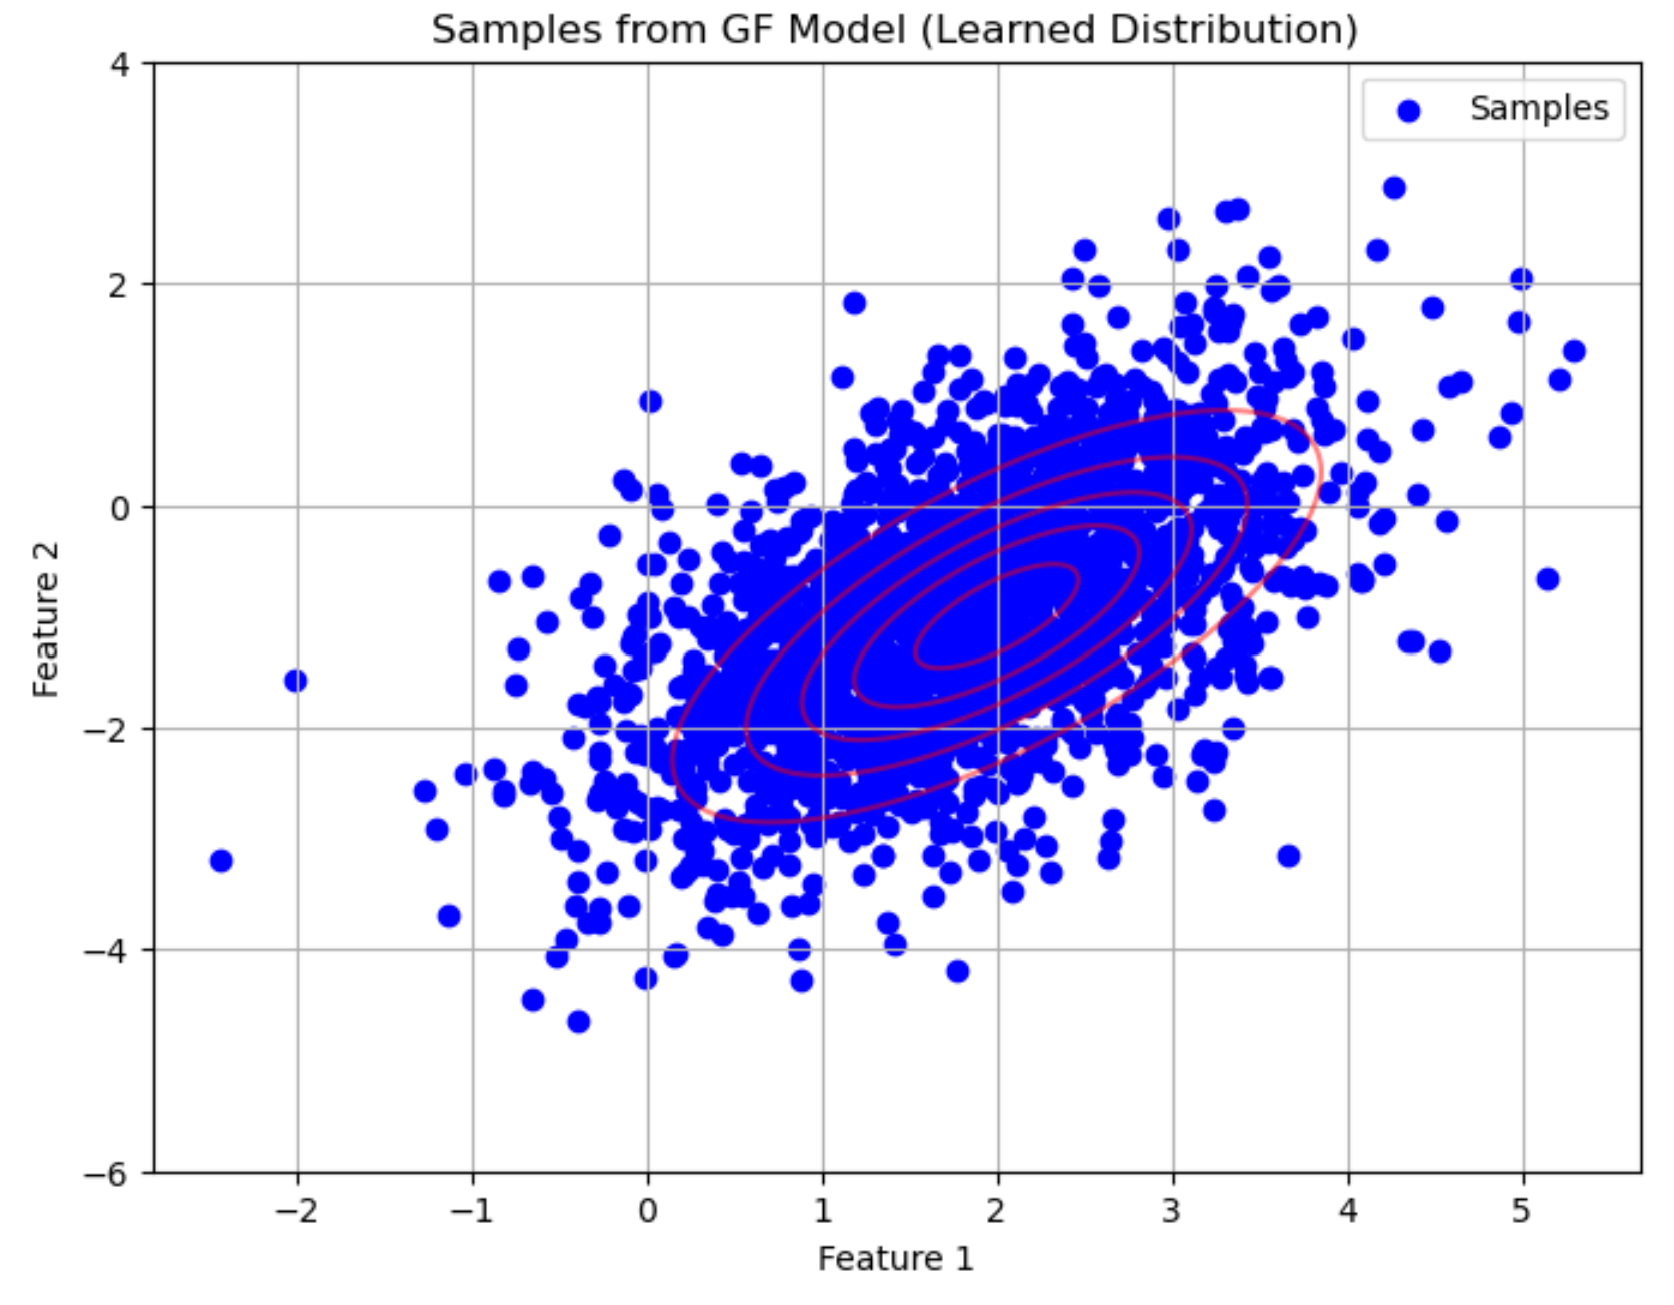
\includegraphics[scale=0.60]{Plots/nf_2d_gaus_2000.png}
\caption{\label{fig:nf_2d_gaus_2000} The first five contours of the true distribution with parameters as in Eqn. \ref{eqn:unimod} in red. The sampled distribution based of the true Gaussian in blue. We sampled 2000 points.}
\end{figure}

Fig. \ref{fig:nf_2d_gaus_2000} shows in red the five first contours of the true distribution with the mentioned parameters in mind (Eqn. \ref{eqn:unimod}). In blue are 2000 points sampled from the true distribution using normalizing flows. The agreement with the true distribution is evident.


\subsection{Multimodal two-dimensional Gaussian}
Now, we wanted to try a multimodal Gaussian distribution in two dimensions. We used the following means

\begin{equation}
    \mu_1 = \begin{pmatrix} 2 \\ -1 \end{pmatrix},\ \mu_2 = \begin{pmatrix} -1 \\ 1 \end{pmatrix},\ \mu_3 = \begin{pmatrix} 1 \\ 3 \end{pmatrix},
\label{eqn:multimod_mean}
\end{equation}

and the following covariance matrices

\begin{equation}
    \mathrm{\Sigma_1} = \begin{pmatrix} 1.0 & 0.5 \\ 0.5 & 1.0 \end{pmatrix},\ \mathrm{\Sigma_2} = \begin{pmatrix} 0.7 & 0.3 \\ 0.3 & 0.7 \end{pmatrix},\ \mathrm{\Sigma_3} = \begin{pmatrix} 1.5 & -0.5 \\ -0.5 & 1.5 \end{pmatrix},
\label{eqn:multimod_cov}
\end{equation}

while weighting the Gaussians according to

\begin{equation}
    \mathrm{w} = (0.4, 0.3, 0.3).
\label{eqn:multimod_weight}
\end{equation}

The result is a sum of two-dimensional Gaussians, weighted with w such that they are properly normalized. Aside from the training data set (800 points), we feature now a validation dataset (200 data points) which should limit overtraining and improve the performance. Also, we compare the Gaussianization Flow with the Neural Spline Flow. We trained the neural net for 25 epochs and compared the results of both flows. As a figure of merit of the performance, we look at the training and validation loss of each flow. \\

\begin{figure}[h!]
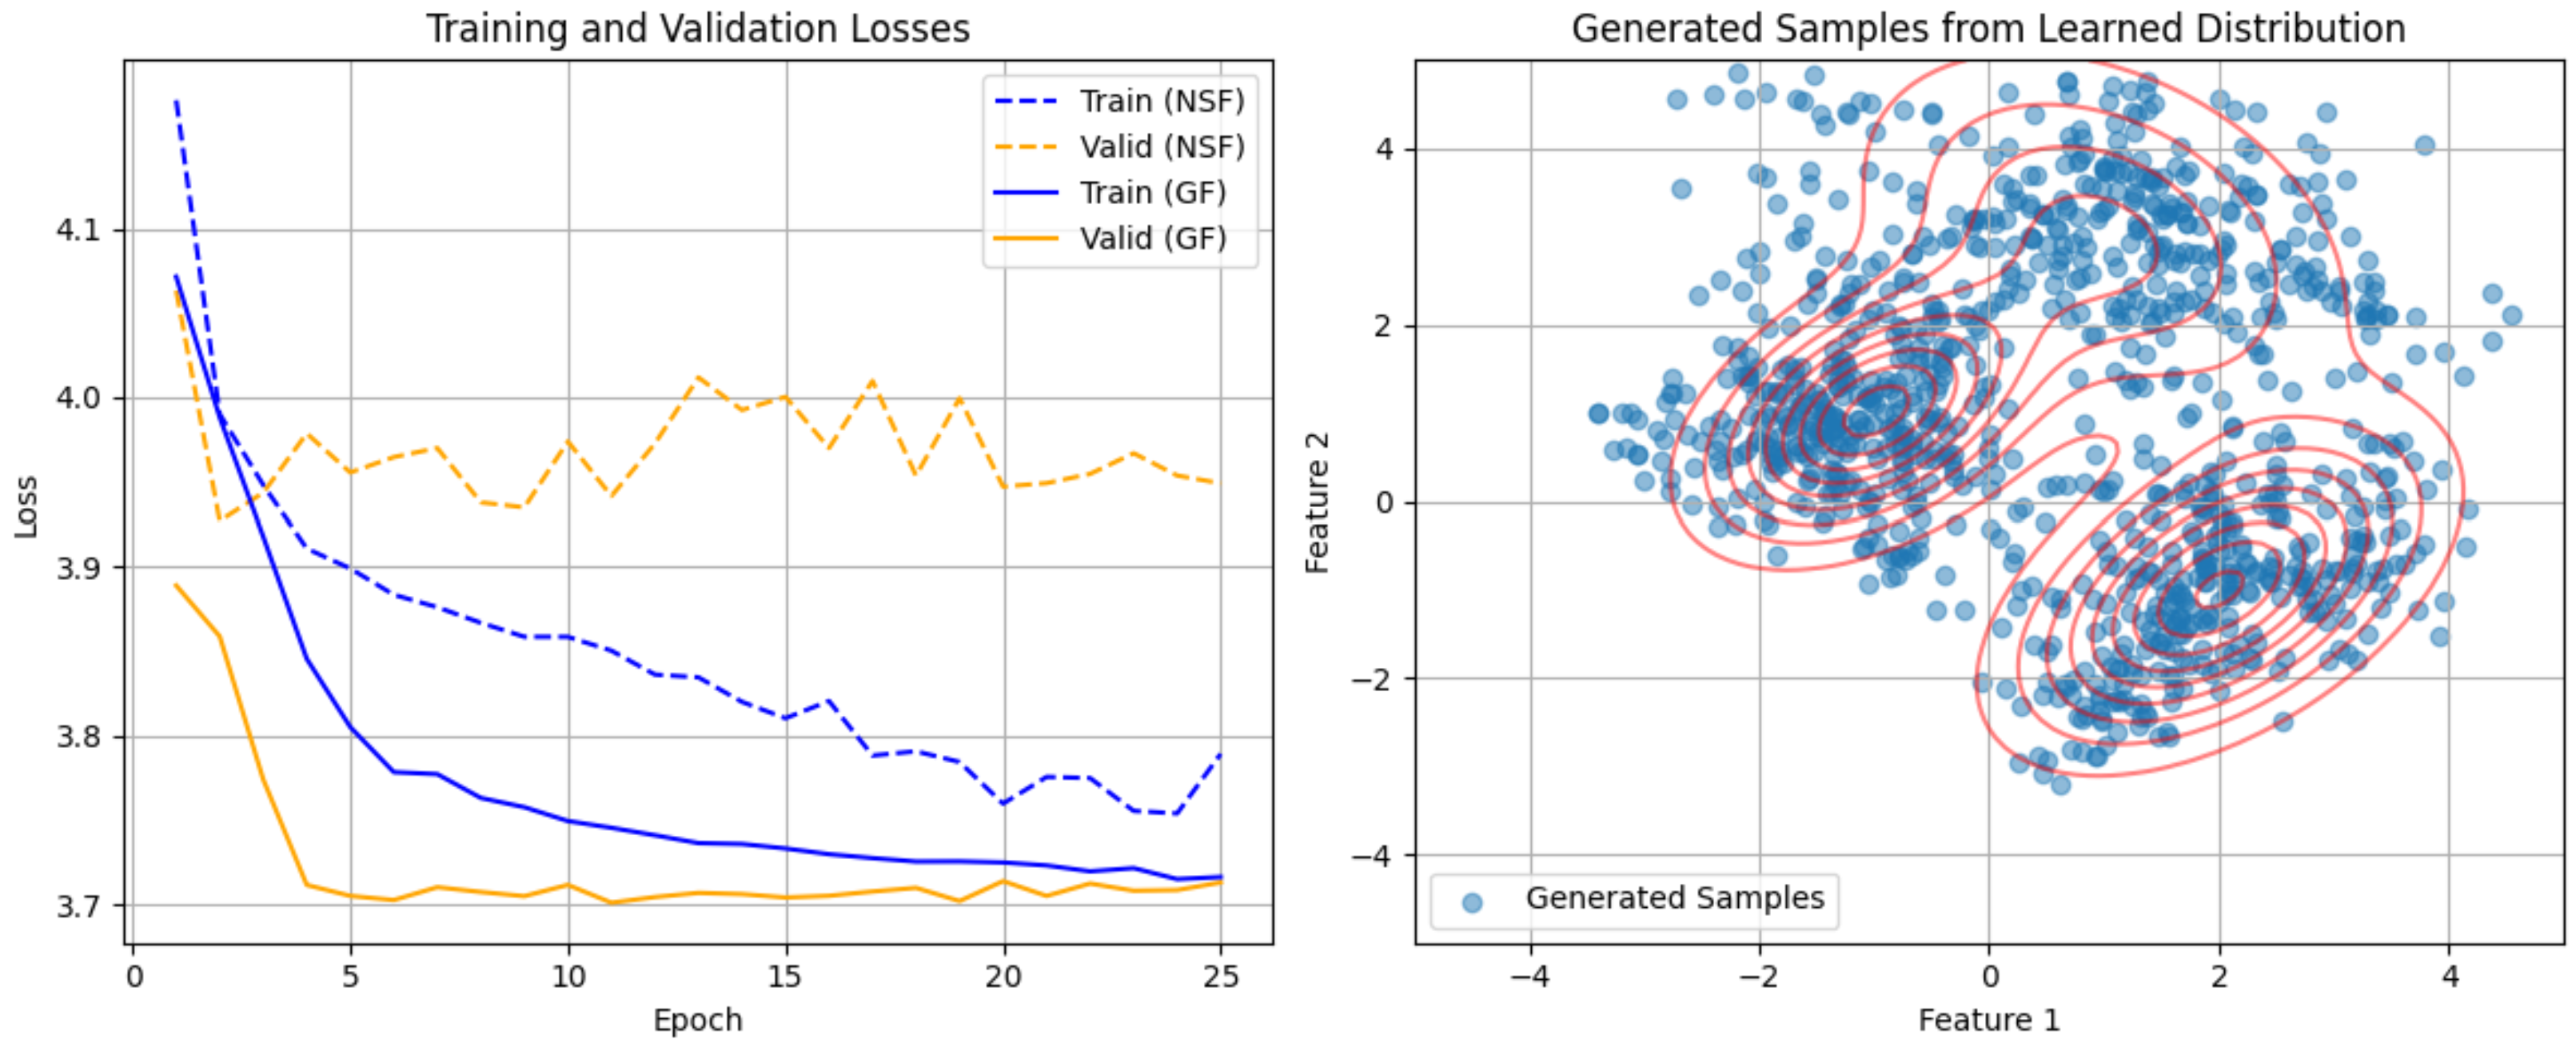
\includegraphics[scale=0.60]{Plots/nf_2d_gaus_multimodal.png}
\caption{\label{fig:nf_2d_gaus_multimodal} The training and validation losses of the NSF and GF algorithm on the left. For the given true distribution of three Gaussians, the GF outperforms the NSF. The sampled distribution with 2000 points on the right with the true distributions contours in red.}
\end{figure}

Figure \ref{fig:nf_2d_gaus_multimodal} shows that in the case of the used multimodal Gaussian function in two dimensions, the Gaussianization Flow is the clear choice. It not only learns the distribution faster (we are dealing with Gaussians after all, so this is expected), its also generalizes best to new, unseen data given the lower training and validation losses. \\

\newpage

\section{Conclusion}
We implemented and tested Normalizing Flows with the \code{zuko} package and compared GF and NSF against each other when considering a trimodal Gaussian function as an input. The GF outperforms the NSF in this special use case given the similar shapes (Gaussian-to-Gaussian, instead of Gaussian-to-Spline). Further studies can be made by considering non-Gaussian functions and see, if the performance stays the same.

\bibliography{bayesian_report} % Produces the bibliography via BibTeX.

\end{document}

